% Created:  Mon 04 Aug 2014 04:49 PM
% @author Josh Wainwright
% File name : add-point-flow.tex

\chapter{Diagrams}
\label{cha:diagrams}

\section{Add-point Flow Diagram}
\label{sec:add_point_flow_diagram}

Figure~\ref{fig:add-point-flow-diagram} is a flow diagram showing the flow of
events from initialisation of the plugin from ImageJ through to drawing the
clusters found to an image of the data set on screen.

\begin{figure*}[tbh]
	\centering
	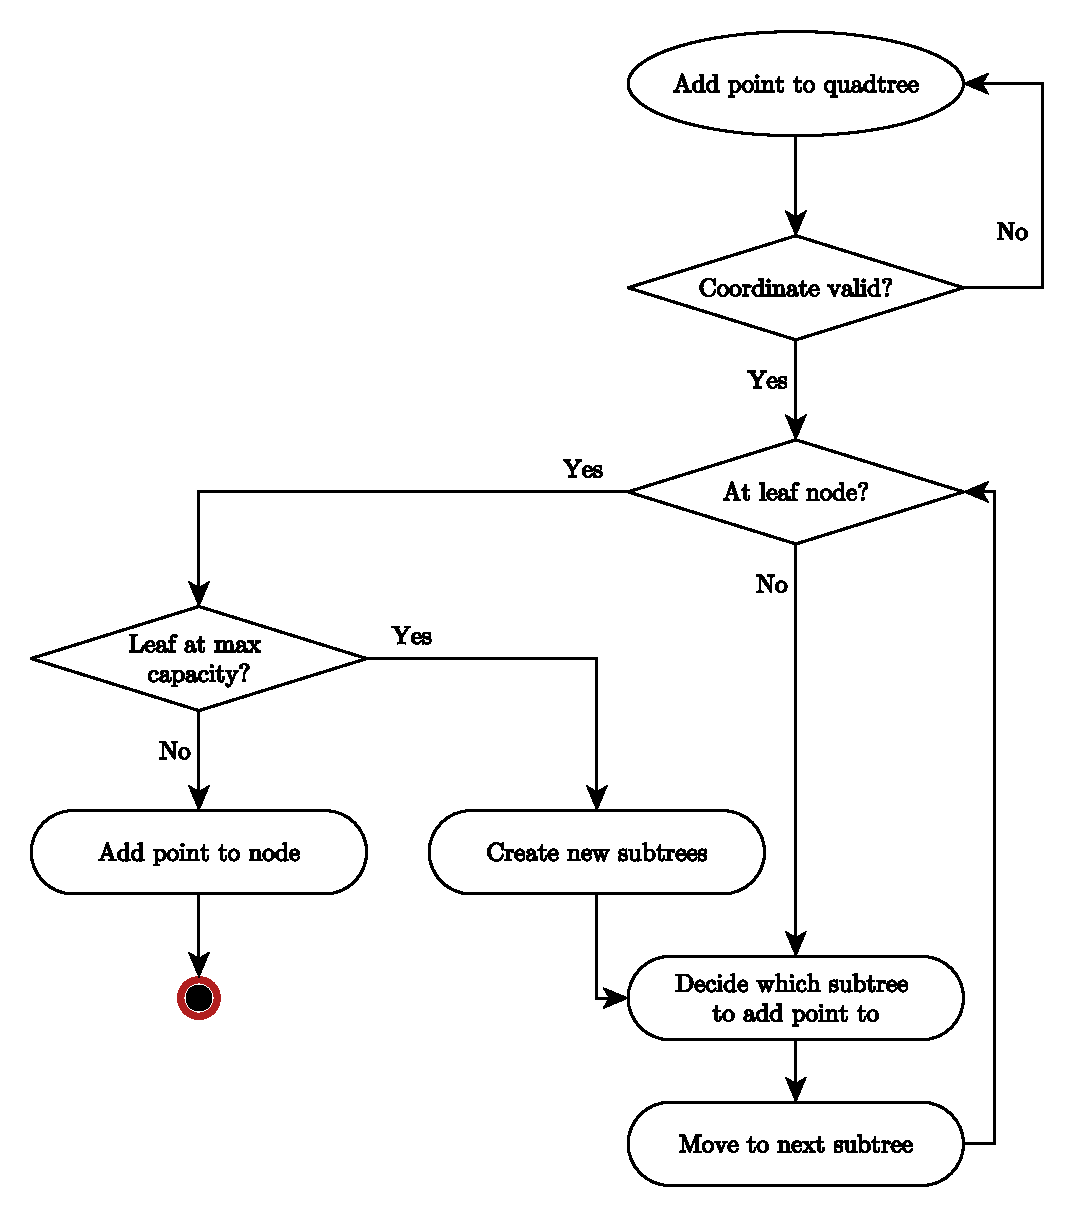
\includegraphics[width=0.8\textwidth]{add-point-flow-chart.pdf}
	% 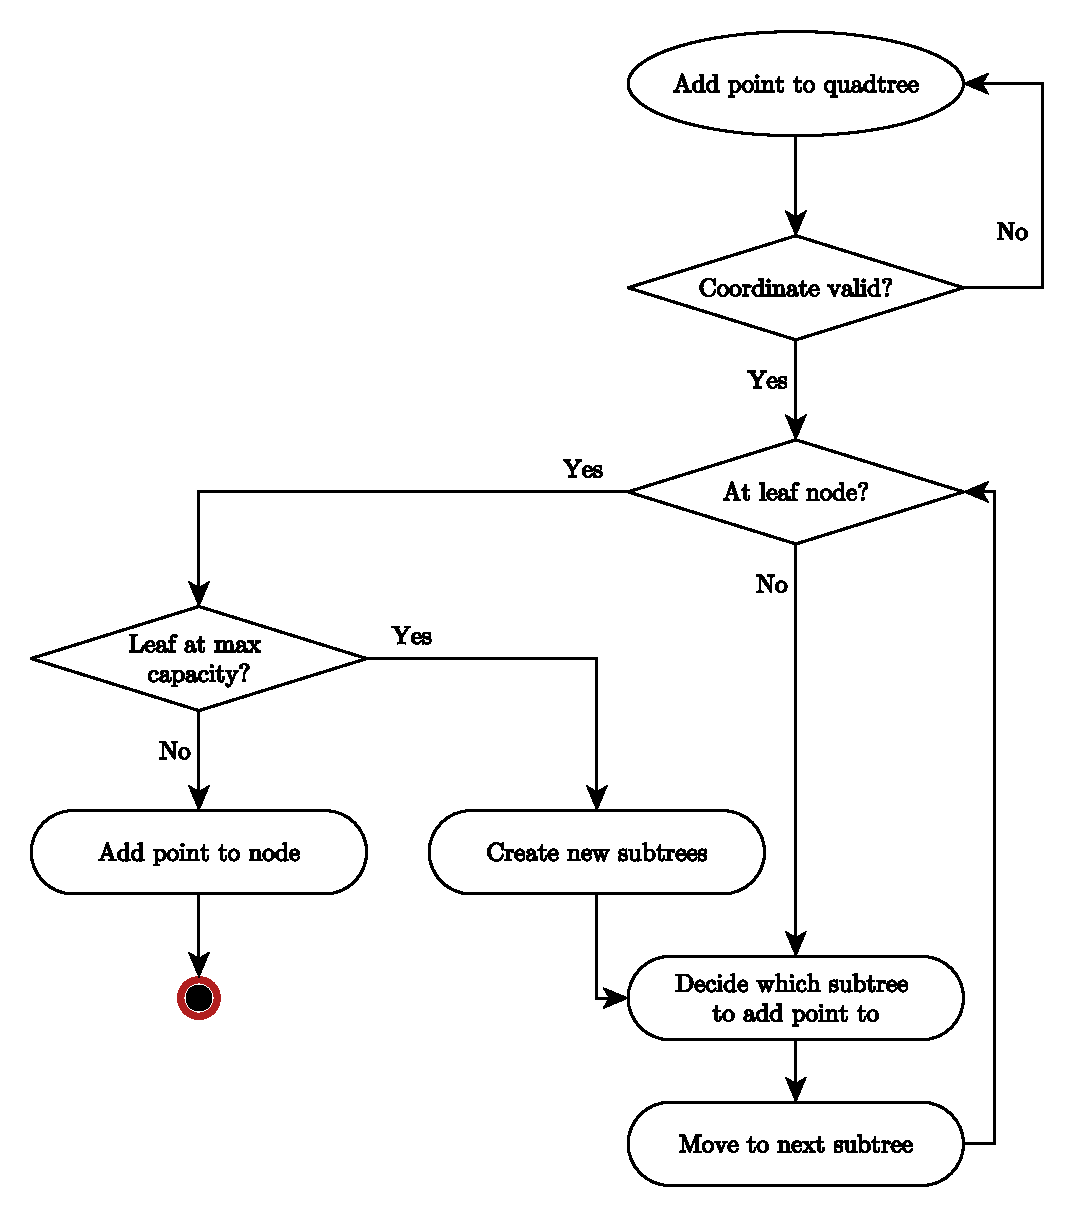
\includegraphics[height=\textheight]{add-point-flow-chart.pdf}

	\caption[Class diagram for the Cluster Analysis ImageJ plugin.]{Class
		diagram for the Cluster Analysis ImageJ plugin written for this
		project.}\label{fig:add-point-flow-diagram}
\end{figure*}
